\chapter{Concurrency in C++}

\section{Threads}

\begin{paracol}{2}
   \begin{figure}[htbp]
      \centering
      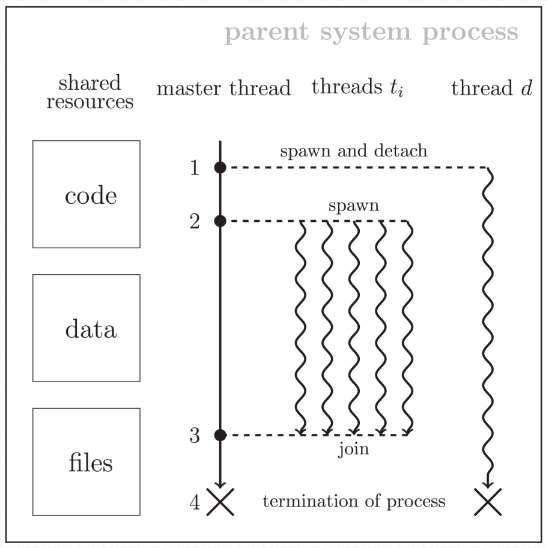
\includegraphics{images/08/threads1.png}
      \caption{Thread schema}
      \label{fig:08/threads1}
   
   \end{figure}
   
   \switchcolumn
   
   \begin{itemize}
      \item The master thread can spawn threads, and each thread can
   spawn threads as well
      \item The number of spawned threads should be roughly the
   amount of cores (i.e., pay attention to oversubscription)
      \item Threads share process resources
      \item each thread has a separate stack
      \item A thread can be joined or detached once
      \item A detached thread cannot be joined
      \item Joined or detached threads cannot be reused
      \item All threads must be joined or detached within the scope of
   their declaration
   \end{itemize}
\end{paracol}


% \begin{lstlisting}[caption={Hello World with threads}, label={lst:08/hello_world}]
% #include <cstdint>
% #include <thread>
% #include <vector>

% // uint64_t
% #include <iostream>  // std :: cout std :: endl
% // std :: vector
% // std: :thread

% // this function will be called by the threads (should be void)
% void say_hello(uint64_t id) {
%   std ::cout << "Hello from thread" << id << std ::endl;
% }
% // this runs in the master thread
% int main(int argc, char* argv[]) {
%   const uint64_t num_threads{(argc == 2) ? std ::stoul(argv[1]) : 10};
%   std ::vector<std ::thread> threads;

%   // for all threads
%   for (uint64_t id = 0; id < num threads; id++)
%     // emplace the thread object in vector threads
%     // using argument forwarding, this avoids unnecessary
%     // move operations to the vector after thread creation
%     threads.emplace_back(
%         // call say hello with argument id
%         say hello, id);

%   // join each thread at the end
%   for (auto& thread : threads) thread.join();
% }
%    \end{lstlisting}

%    \begin{itemize}
%       \item We need to store the thread handles explicitly to be able
%       to access them during the join phase
%       \item In the code snippet, we use a \lstinline|std::vector| container and
%       the method \lstinline|emplace_back|
%       \item Alternatively, we could have moved the thread object
%       implicitly using the vector member function \lstinline|push_back|
%       \item \lstinline|threads.push_back(std :: thread(say_hello, id));|
%       \item The type std::thread is move-only (i.e., not copyable)
%       \item How to compile:
%       \item \lstinline|g++ -O2 -std=c++17 hello_world.cpp -o hello_world -pthread|
%    \end{itemize}
   
\section{Asynchronicity and Tasks}
It may be more convenient to let the threads start asynchronously. This can be achieved by using the \lstinline|std::async| function. This function returns a \lstinline|std::future| object that can be used to retrieve the result of the function. The function is executed asynchronously, and the result is stored in the \lstinline|std::future| object. The function \lstinline|std::future::get()| can be used to retrieve the result. The function \lstinline|std::future::wait()| can be used to wait for the result to be available. The function \lstinline|std::future::valid()| can be used to check if the result is available. 

Note however that a call to \lstinline|std::async| \ul{does \textit{not} necessarily imply that a new thread is spawned.}
The calling thread might execute the task without spawning a thread!\\
Default behavior depends on the implementation; thus, remember to use \lstinline|std::launch::async|
\begin{lstlisting}
   auto future = std::async(std::launch::async, foo, id);
\end{lstlisting}

\subsection{Tasks}
The \lstinline|std::package_task| function that allows you to conveniently
construct task objects, which are callable objects (function pointer, functor class, member function pointer, lambda,
std::function wrapper, …) with associated the corresponding future object handling the return value

\dots

% //TODO

\section{Mutexes}
A mutex is a synchronization mechanism that guarantees mutual exclusion execution of a critical
section. Its usage restricts the execution of a critical section to a single thread at a time.\\
A thread locking a mutex prevents other threads from acquiring the mutex. The other threads wait for
its release (passive waiting).

\begin{paracol}{2}
   
   \begin{lstlisting}
#include <mutex>
std: :mutex mutex;
// to be called by threads
void some_function ( ... ) {
   mutex. lock ()
   // this region is only processed by one thread at a time
   mutex. unlock() ;
   // this region is processed in parallel
}
   \end{lstlisting}

   \switchcolumn

   \begin{lstlisting}
#include <mutex>
std: : mutex mutex;
// to be called by threads
void some_function ( ... ) {
   // here we acquire the lock
   std :: lock_guard<std: :mutex> lock_guard(mutex);
   // this region is locked by the mutex
   } // <- here we release the lock
   // this region is processed in parallel
}
   \end{lstlisting}
\end{paracol}

\subsection{Different implementations}
\begin{itemize}
	\item \lstinline|std::lock_guard| is a wrapper around \lstinline|std::mutex| that acquires ownership of the mutex upon
construction and releases it upon destruction.
   \begin{itemize}
      \item Once constructed, it cannot be explicitly released until it goes out of scope
      \item It can only manage a single mutex
   \end{itemize}
      \item \lstinline|std::scoped_lock| manages multiple mutexes simultaneously, acquiring/releasing all of them
      simultaneously when entering/exiting the scope.
      \begin{itemize}
         \item It provides an \lstinline|unlock()| method to explicitly release the locks before the end of the scope.
         \item Helps avoid deadlock when you need to acquire multiple locks together
         \item Pay attention to the fact that it accepts 0 mutexes, resulting in a run-time error
      \end{itemize}
\end{itemize}

\subsection{Condition Variables}
A CV enables one or more threads to wait (passively) for an event inside a critical section.

Conceptually, a CV is associated with an event or condition. When a thread has determined that the condition is satisfied,it can notify one or more of the threads waiting on the CV to wake them up.

Pay attention to \textbf{spurious wake-ups}! The condition must be checked in a loop (typically a while loop).

\section{Distributing Workload}

\subsection{Static assignment}
We may distribute the work in various manners.
A possibility is to assign a fixed number of elements to each thread. This is called \textbf{static assignment}.
Supposing an array of data $b = {b_0, b_1, \ldots, b_15}$ and $p=5$ processors, these are three common strategies:
\begin{paracol}{2}
   \begin{itemize}
      \item \textbf{Block distribution}: Each processor gets a block of data. For example, $p_0$ gets $b_0, b_1, b_2, b_3$; $p_1$ gets $b_4, b_5, b_6$; and so on.
      \item \textbf{Cyclic distribution}: Each processor gets every $p^th$ element. For example, $p_0$ gets $b_0, b_5, b_{10}, b_{15}$; $p_1$ gets $b_1, b_6, b_{11}$; and so on.
      \item \textbf{Block-cyclic distribution} given $c$ block size: A combination of the two above. For example, $p_0$ gets $b_0, b_1, b_{10}, b_{11}$; $p_1$ gets $b_5, b_6, b_{12}, b_{13}$; and so on.
      \note{$c\cdot p$ is called \textbf{stride}. $b_i$ is assigned to $p_{(i/c)\ mod\ p}$ }
   \end{itemize}

\switchcolumn

\begin{figure}[htbp]
   \centering
   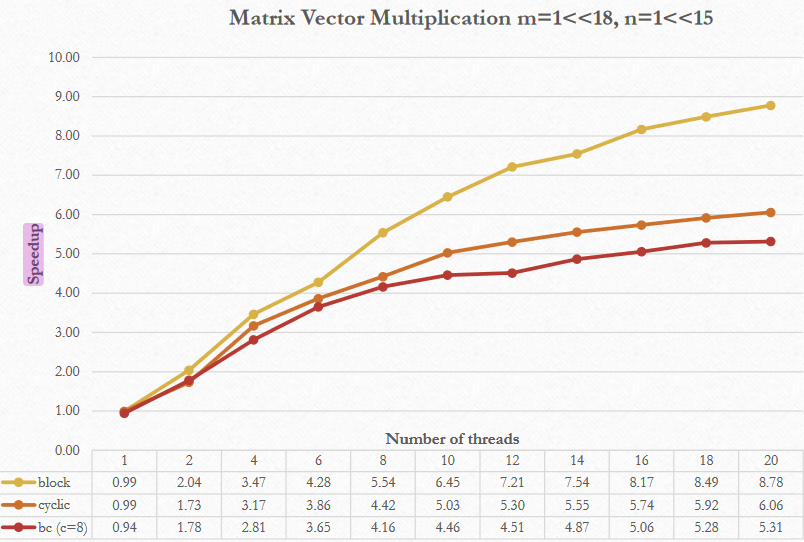
\includegraphics{images/08/speedup}
   \caption{Speedup comparison}
   \label{fig:08/speedup}
\end{figure}

\end{paracol}

\begin{figure}[htbp]
   \centering
   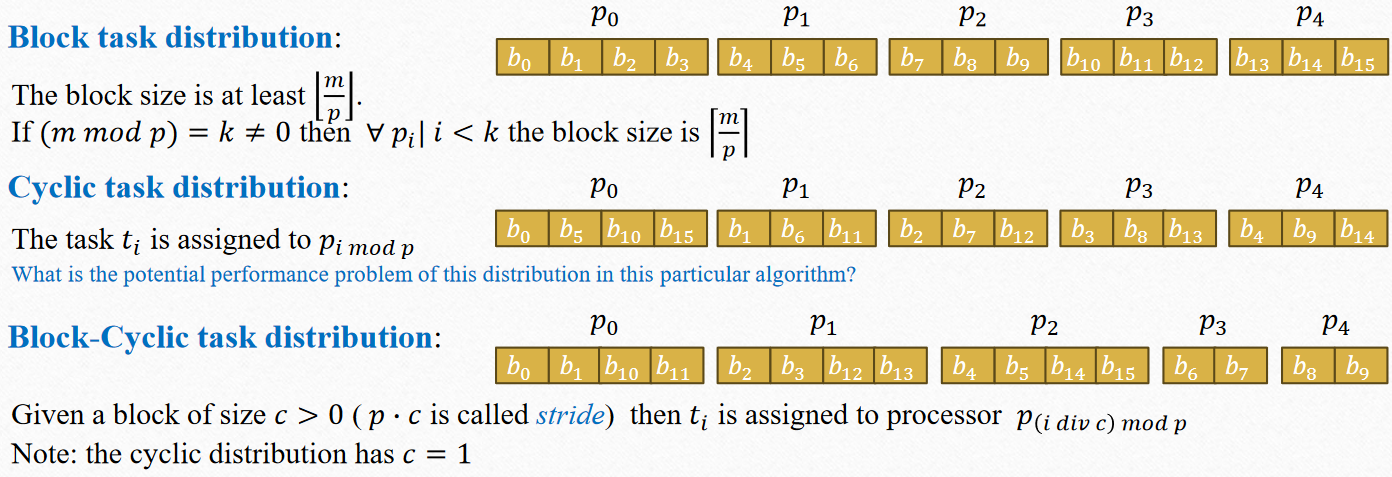
\includegraphics{images/08/static}
   \caption{Static assignment strategies}
   \label{fig:08/static}
\end{figure}

\subsection{Dynamic assignment}

It may not be possible to know in advance how much work each task will have to do. 
The size of the problem may be unkown, or the workload may be unbalanced, meaning that some tasks may result in more work than others.
Even in the case of multiplying matrices, the workload may be strongly unbalanced if the matrices are sparse.

For such cases, dynamic assignment is more appropriate. The master thread assigns work to the worker threads as they become available. This is done by using a \textbf{work queue}.

\framedt{All-pairs distance Matrix}{
   \begin{itemize}
      \item We have a $m\times n$ matrix $D_{ij}$ where $i$ denotes one of the $m$ vectors and $j$ enumerates the $n$ elements of the vector.
      \item We want to compute the distance (or \textit{similarity}) $d(\cdot,\cdot)$ between all pairs of vectors.
      \begin{itemize}
         \item $\Delta_{ij} = d(x^{(i)}, x^{(i')}) \quad = \sqrt{\sum_{k=1}^{n} (D_{ik} - D_{jk})^2}$
         \item The distance/similarity measure $d(\cdot,\cdot)$ might be a traditional metric such as Euclidean distance or any symmetric binary function that assign a notion of similarity to pair of instances
      \end{itemize}
      \item We have to comput $m^2$ distances, so $\mathcal{O} (m^2n)$ operations
      \item However note that $\Delta_{ij} = \Delta_{ji}$, i.e. it is a symmetric matrix, so we can compute only the lower triangular part
   \end{itemize}
}

\begin{paracol}{2}
   We statically assign each row to a thread, using a block cycling distribution.
   This is not ideal, as some rows may take longer to compute than others, resulting in unbalanced workloads.

   In Fig. \ref{fig:08/delta_static} we can see the distribution of the workload. Each row is assigned to a thread, and the workload is distributed in blocks size $c = 2$.
   As $c$ increases, the number of blocks decreases, and the workload becomes more unbalanced.

   \switchcolumn

   \begin{figure}[htbp]
      \centering
      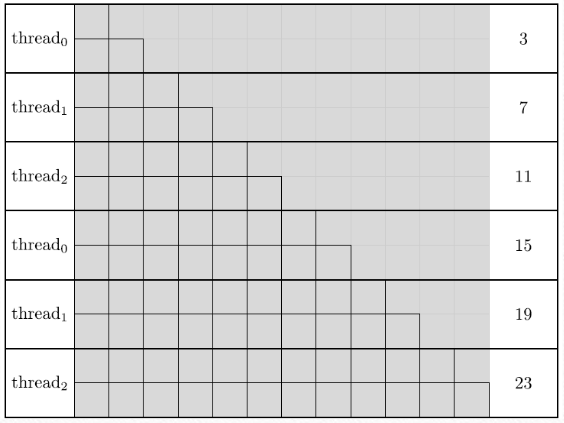
\includegraphics{images/08/delta_static.png}
      \caption{Block cyclic distribution}
      \label{fig:08/delta_static}
   \end{figure}
\end{paracol}

\begin{paracol}{2}
   Consider the snippet on the right. Each thread tries to hold a lock on the mutex, and then updates the global variable \lstinline|lower| with the next row to compute. The global variable \lstinline|global_lower| is updated by the master thread.

   This is a simple example of dynamic assignment, directly performed by thread and automatically balancing the workload. This however comes at the cost of the mutex overhead, which is not negligible.

   In general, if the \ul{workload is not-so-unbalanced, static assignment is preferable}.
   
   \switchcolumn

   \begin{lstlisting}[caption={spm3/all-pairs.cpp}]
// while there are still rows to compute
while (lower < rows) {
   
   // update lower row with global lower row
   {
      std::lock_guard<std::mutex> lock_guard(mutex);
      lower  = global_lower;
      global_lower += chunk_size;
      }
   \end{lstlisting}
         
\end{paracol}


\subsubsection{Producer-Consumer model}
Here we have a shared data structure, typically a queue, that is accessed by multiple threads. The producer thread(s) insert data into the queue, while the consumer thread(s) remove data from the queue. The producer and consumer threads are synchronized by a mutex and a condition variable.

\paragraph{Stop token}

The \lstinline|std::stop_token| is a mechanism to signal the threads to stop. The producer thread will keep adding data to the queue until the stop token is requested. The consumer thread will keep consuming data from the queue until the stop token is requested.

It is not always the way-to-go solution to stop threads, it is one of the available options.
Another option is to use a global \lstinline|std::atomic<bool>| flag, which is more efficient but less flexible.
Or, as I did in my Operative Systems project, to insert a \textit{special value} in the queue to signal the end of the data. 
   
   \begin{lstlisting}[caption={spm3/prod-cons.cpp}]
std::stop_token stoken = stopSrc.get_token();
// ...
auto producer = [&](const std::stop_token &stoken, int id) {	   
	uint64_t i=0;
	while (!stoken.stop_requested()) {
		{
			std::lock_guard<std::mutex> lock(mtx);
			dataq.push_back(i++);
		}
		cv.notify_one();
      //...

auto consumer = [&](const std::stop_token &stoken, int id) {
	std::unique_lock<std::mutex> lock(mtx, std::defer_lock);
	for(;;) {
		lock.lock();
		if (cv.wait(lock, stoken, [&dataq] { return !dataq.empty(); })) {
			auto data = dataq.front();
			(void)data;
			dataq.pop_front();
			//std::printf("Consumer%d, data=%lu\n", id, data);
		}
		else {
			if (stoken.stop_requested()) {
				lock.unlock();
				break;
			}
		}
		lock.unlock();
      // ...
\end{lstlisting}

\newpage
\subsubsection{Multiple-Reader Single-Writer}

A reader may access the data concurrently with
other readers, while a writer needs exclusive access to the shared data.
This is a common pattern with a simple  ---not trivial--- solution.

\begin{paracol}{2}
   
   \colfill
   Using a normal \lstinline|std::mutex| to protect the accesses to the critical section \textbf{does prevent} the concurrent access of multiple readers, so it is not a viable solution.
   The Standard library offers a solution with \lstinline|std::shared_mutex|, which allows multiple readers to access the data concurrently, while a writer needs exclusive access to the shared data.
   \colfill
   
   \switchcolumn   
   
   \begin{lstlisting}[caption={spm3/reader-writer.cpp}]
auto reader = [&](int count, int id) {
   for(int i=0;i<count; ++i) {
      std::shared_lock<std::shared_mutex> lock(smutex);
      std::printf("Reader%d has read %d\n", id, shared_counter);
   }
};
auto writer = [&](int count, int id) {
   for(int i=0;i<count; ++i) {
      std::unique_lock<std::shared_mutex> lock(smutex);
      ++shared_counter;
      std::printf("Writer%d has written %d\n", id, shared_counter);
   }
};  
\end{lstlisting}
               
\end{paracol}

\subsubsection{Thread Pool}
Instead of creating threads on the fly, we can create a pool of threads that are ready to execute tasks. This is useful when the overhead of creating threads is high, and we want to reuse threads for multiple tasks.

There is no out-of-the-box solution of a Thread Pool (TP) in the Standard Library. There are many libraries that provide thread pools, such as \textit{Boost} or \textit{Intel TBB}, but we can also manage them by ourselves.

The synchronization is handled through mutex and condition variables, in a Producer-Consumer fashion.
In the \ul{implementation provided (\texttt{threadPool.hpp}) the task queue is \textbf{unbounded}!}
If the producers are much faster than the Workers, the tasks queue becomes huge, and the memory blows up \frownie.\\
To avoid this we can either increase the number of Worker threads (if we have enough cores), or we can implement a \textbf{bounded queue}.